Android est un système d'exploitation open source crée principalement pour les appareils mobiles et 
les tablettes tactiles. Le système d'exploitation basé sur Linux est dirigé par l'entreprise Google
depuis 2005. Il possède une surcouche utilisant le langage Java sur lequel tourne les applications 
Android.
Aujourd'hui, Android est l'OS le plus utilisé dans le monde sur les téléphones portables.



%%%%%%%%%%%%%%%%%%%%%%%%%%%%%%%%%%%%%%%%%%%%%%%%%%%%%%%%%%%%%%%%%%%%%%%%%%%%%%%%%%%%%%%%%%%%%%%%%%%%
\subsection{Fonctionnement global}
%%%%%%%%%%%%%%%%%%%%%%%%%%%%%%%%%%%%%%%%%%%%%%%%%%%%%%%%%%%%%%%%%%%%%%%%%%%%%%%%%%%%%%%%%%%%%%%%%%%%



Le fonctionnement global du projet sur la plateforme Android est relativement simple. Nous souhaitons
simplement pouvoir utiliser le téléphone portable comme un intermédiaire entre notre site web et le 
correspondant avec qui nous discutons. Pour cela le téléphone fait office de proxy entre les deux 
entités éloignés. Un proxy est un composant qui se place entre un interlocuteur et sont auditeur. Le 
proxy sert principalement à relayer l'information d'un élément vers un autre, il sert d'intermédiaire.
Dans notre cas, le proxy s'occuppe de recevoir des SMS et de les rediriger vers le site web. 
Réciproquement, il récupère les messages envoyés par le site web et envoie un SMS vers le correspondant
définis dans le message reçu.



%%%%%%%%%%%%%%%%%%%%%%%%%%%%%%%%%%%%%%%%%%%%%%%%%%%%%%%%%%%%%%%%%%%%%%%%%%%%%%%%%%%%%%%%%%%%%%%%%%%%
\subsection{Création du service}
%%%%%%%%%%%%%%%%%%%%%%%%%%%%%%%%%%%%%%%%%%%%%%%%%%%%%%%%%%%%%%%%%%%%%%%%%%%%%%%%%%%%%%%%%%%%%%%%%%%%



Les applications fonctionnant sous Android régissent par un principe simple, celui des "activités".
Pour simplifier, une activité représente une fonctionnalité graphique d'une application. Par exemple,
lorsqu'une application est ouverte, on tombe sur un menu avec les différentes possibilités d'actions 
qui nous sont offertes. Le menu représente donc ici une activité. 
\\


Il faut savoir que une activité lorsqu'elle est active occupe le système qui attend des évènements.
Si l'utilisateur ne fait rien alors que le menu est affiché, le système peut s'occupper d'autres 
taches annexes. Si en revanche l'utilisateur navigue dans le menu, alors l'activité est considérée
comme en fonctionnement et bloque toute autres opérations non relative à l'application executée.
\\


Dans le cadre de notre application, nous devons à son lancement effectuer une série d'opérations 
afin de mettre l'application en fonctionnement. Cela consiste notamment à, vérifier l'état de la 
connectivité internet, récupérer les identifiants et se connecter sur le service GTalk. Ces 
opérations rende le système bloquant durant leur exécutions. Cela n'est pas un problème lorsque la 
connection s'effectue sans erreurs. Le traitement durant moins d'une seconde, le système n'est pas
gravement impacté. En revanche, si une erreur intervient, le programme va alors essayer de la résoudre.
Cela n'est pas concevable. En effet, une perte soudaine de réseau pourrait par exemple mettre 
l'application dans un état de recherche ce qui est potentiellement très lent. Cette situation rendrait
le terminal complètement blocké durant la recherche. 

Ce comportement n'étant pas souhaitable, nous avons du trouver une solution pour pouvoir outrepasser ce blocage.
\\


Nous avons alors utilisé le concept Android de "services". Celui-ci consiste à executer une fonctionnalité 
de manière asynchrone. Le service n'impacte pas le système, au contraire il fonctionne avec lui. 

\begin{figure}[!h]
	\center
	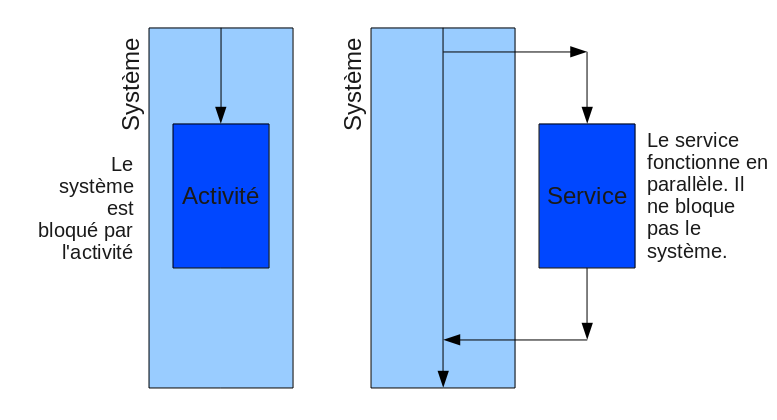
\includegraphics[width=13cm]{img/fonctionnement-des-services-android.png}
	\caption{fonctionnement d'un service Android}
\end{figure}

Comme montré ci-dessus, le service n'est pas  bloquant. Lors de son éxecution, le système continue de 
fonctionner sur d'autres taches en paire avec le service lancé.
\\\\
Dans notre cas, le service sert à deux taches principales. Tout d'abord il va configurer l'authentification
de l'utilisateur sur GTalk. Ensuite il va simplement se mettre en attente d'évènement et le cas échéant, 
traiter ce meme évènement.




%%%%%%%%%%%%%%%%%%%%%%%%%%%%%%%%%%%%%%%%%%%%%%%%%%%%%%%%%%%%%%%%%%%%%%%%%%%%%%%%%%%%%%%%%%%%%%%%%%%%
\subsection{Authentification sur GTalk}
%%%%%%%%%%%%%%%%%%%%%%%%%%%%%%%%%%%%%%%%%%%%%%%%%%%%%%%%%%%%%%%%%%%%%%%%%%%%%%%%%%%%%%%%%%%%%%%%%%%%



Pour pouvoir relayer communiquer avec le site web, notre projet utilise le protocole XMPP. Plus 
précisément, nous utilisons un meme et unique compte GTalk. 

Initialement, le projet devait etre conçu pour Android. Or chaque utilisateur Android a un compte 
gmail. Ce meme compte peut etre utiliser pour accéder à tous les services de Google dont GTalk.
C'est une des raisons qui a fait que nous avons choisi XMPP plutot qu'un autre protocole. L'utilisateur
n'a ainsi pas besoin de créer quelquonque nouveaux comptes et peux utiliser celui qu'il possède déja.
\\


Pour pouvoir converser avec le site web, l'application a besoin de s'authentifier auprès du service
GTalk. Pour cela, nous sommes passés par deux étapes. 

Initialement, nous utilisions la méthode classique d'authentification. Lorsque l'utilisateur lance 
l'application, celle-ci lui demande de rentrer ses identifiant et mot de passe. Cela effectué, 
l'application se charge de se connecter et de s'authentifier sur les serveurs GTalk en utilisant les
paramètres rentrés par l'utilisateur.

Cette solution qui est la plus simple à implémenter mais n'est malheureusement pas la plus agréable
à utiliser ni la plus sure. Nous forçons en effet l'utilisateur à rentrer ses identifiants ce qui 
pourrait paraitre légitime mais reste contraignant pour l'utilisateur. Celui-ci ne sait pas ce que 
nous faisons avec son mot de passe. Une application malveillante pourrait récupérer les identifiants
et s'en servir à des fins illégales. Dans notre cas, meme si nous n'avions aucune mauvaise intentions,
nous ne pouvons demander aux utilisateurs de nous faire confiance. Nous avons donc opté pour une 
deuxième solution, l'identification avec OAuth2.0.

Comme vu précédement, OAuth permet de réaliser des actions en agissant à la place de l'utilisateur. 
Ici nous souhaitions simplement utiliser le compte GTalk de l'utilisateur sans que celui-ci ai à rentrer
ses identifiants. 

Le fonctionnement est simple. Lorsque utilisateur lance l'application, celle-ci demande tout d'abord
à l'utilisateur quel compte gmail il veut utiliser parmi ceux présent sur sont téléphone. Dans le cas
ou il n'existe qu'un seul compte, celui-ci est choisi par défaut.
\\


Suite à cela, le protocole OAuth va demander à l'utilisateur une seule et unique fois si il authorise 
l'application à accéder à son compte GTalk. La validation effectué, l'application pourra se connecter 
à chaque lancement, automatiquement et sans importuner l'utilisateur. 
\\


Contrairement a l'authentification sur le site web, l'authentification sur une plateforme android est
théoriquement plus simple. En effet, une fois que l'utilisateur a donné son accord, le server 
d'authentification de google va directement envoyer le token d'authentification. Il n'y a alors pas 
besoin d'effectuer une deuxième étape pour récupérer ce dernier.

%%%%%%%%%%%%%%%%%%%%%%%%%%%%
%title Envoi d'un SMS

%Utilisateur->Application: dégation de l'authentification
%Application->Serveur google: requete pour un token d'authentification
%Serveur google->Application: token d'authentification
%Application->serveur gtalk: authentification(token)
%serveur gtalk->Application: authentification validé
%%%%%%%%%%%%%%%%%%%%%%%%%%%%

\begin{figure}[!h]
	\center
	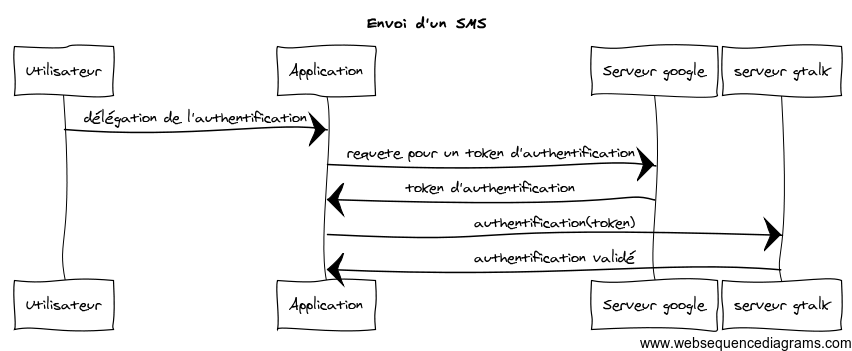
\includegraphics[width=15cm]{img/obtention-token-avec-android.png}
	\caption{procédure d'obtention d'un token avec un appareil Android}
\end{figure}

Néanmoins, une des difficultés d'implémenter ce protocole est que la libraire de gestion de compte
XMPP pour Android dénommé Asmack est différente de celle utiliser pour le site web. Asmack est un fork 
de la librairie Smack pour Android et est l'unique librairie gérant les comptes XMPP présente sur
Android. Ne souhaitant pas réimplémenter toute les fonctionnalités présentes dans celle-ci, nous avons
choisi de l'utiliser. Malheuresement, les différences entre les deux librairies nous ont empechés de 
réimplementer notre précédent travail effectué pour le site web qui était fonctionnel. 

Le langage Java fonctionne sur une machine virtuelle. Celle-ci contient des fonctionnalités basique sur
lesquelles le langage peut s'appuyer. Dalvik, la machine virtuelle pour Java présente sur Android n'est 
pas exactement la meme que la machine virtuelle basique. En effet, pour des soucis de rapidité et de 
légèreté, certaines parties de Dalvik ont été réécrites pour en faire une machine virtuelle plus adapté
aux plateformes mobiles.

Smack a été développé sur la machine virtuelle Java basique tandis que Asmack a été développé sur Dalvik.
Cette différence implique des changements quand aux fonctionnements de celles-ci. 

Finalement, en réimplémentant certaines fonctionnalités, nous avons réussi à nous authentifier avec OAuth.
\\


Authentifier un utilisateur via OAuth2.0 sur Android a était un réel challenge. Il nous a fallu comprendre 
et trouver des équivalences au fonctionnement de Smack. 



%%%%%%%%%%%%%%%%%%%%%%%%%%%%%%%%%%%%%%%%%%%%%%%%%%%%%%%%%%%%%%%%%%%%%%%%%%%%%%%%%%%%%%%%%%%%%%%%%%%%
\subsection{Envoi et réception d'un SMS}
%%%%%%%%%%%%%%%%%%%%%%%%%%%%%%%%%%%%%%%%%%%%%%%%%%%%%%%%%%%%%%%%%%%%%%%%%%%%%%%%%%%%%%%%%%%%%%%%%%%%


\subsubsection{Réception d'un SMS}

Une fois authentifié, nous souhaitons pouvoir utiliser notre téléphone comme proxy. Notre application
doit en effet servir d'intermédiaire entre le site web et un correspondant. Pour cela elle doit tout
d'abord surveiller l'arrivée de nouveaux messages. 

Sur Android, le monitoring d'évènements n'implique pas de devoirs sortir des sentiers battus. En effet,
des outils mis en place par Google authorise la surveillance du comportement du téléphone. Dans notre cas 
nous avons pu utiliser le principe de "Broadcast Receiver" du système. 

Un broadcast receiver est un outils qui permet de rendre une application consciente de son environnement.
Cela permet généralement à l'application qui l'utilise d'etre prévenu lors de nouvelles notifications ou 
d'un comportement particulier du téléphone.
Son fonctionnement est simple. Il permet de s'enregistrer auprès du téléphone qui maintient une base de donnée des 
membres à avertir lors d'un changement particulier.

\begin{figure}[!h]
	\center
	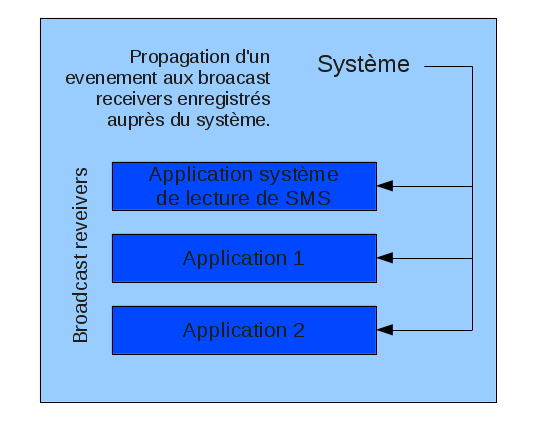
\includegraphics[width=12cm]{img/broadcast-receivers.png}
	\caption{fonctionnement des broadcasts receivers sur Android}
\end{figure}

Ci dessus, on peut voir le système du téléphone qui contient les différents broadcast receiver à avertir
en cas de nouveaux messages. Ici l'application de rédaction de SMS ainsi que deux autres applications seront
avertis.

Dans notre cas, nous nous en sommes servis pour d'une part etre avertis de l'arrivé de nouveaux SMS et d'autre 
part pour pouvoir récupérer le dit message et le traiter.
\\


\subsubsection{Envoi d'un SMS}

L'envoi quand à lui est beaucoup plus trivial. Android met à disposition un outils permettant d'envoyer
des messages.


%%%%%%%%%%%%%%%%%%%%%%%%%%%%%%%%%%%%%%%%%%%%%%%%%%%%%%%%%%%%%%%%%%%%%%%%%%%%%%%%%%%%%%%%%%%%%%%%%%%%
\subsection{Traitement des évènements}
%%%%%%%%%%%%%%%%%%%%%%%%%%%%%%%%%%%%%%%%%%%%%%%%%%%%%%%%%%%%%%%%%%%%%%%%%%%%%%%%%%%%%%%%%%%%%%%%%%%%



\subsubsection{Architecture de l'application}

Pour pouvoir réagir en fonction d'un évènement, notre application a successivement adopté deux méthodes.

La première a été réalisé pour répondre aux besoins de notre projet. Il s'agissait d'un test sur le 
type de l'évènement entrant. Plus précisément, il s'agissait de vérifier si l'évènement en question 
était la récéption d'un nouveaux SMS ou bien la récéption d'un nouveau message XMPP en provenance du 
site web. En fonction du type de message en entrée, l'application décidé d'envoyer transmettre le message
vers le bon destinataire. 

Ce fonctionnement basique convenait totalement à nos besoins mais par soucis de rendre notre application
évolutive nous avons travaillé sur une deuxième solutions.

Lors de la réception d'un message XMPP, nous souhaitions pouvoir réagir différement en fonction du contenu
du message. Dans le cadre de notre projet, nous n'avions comme but que l'envoi de sms à partir du webservice
seulement. Notre travail respecté donc ce principe mais ne permettait aucune évolutivité.

A supposer qu'un tiers soit intéressé par la communication entre le webservice et le téléphone par 
l'intermédiaire de XMPP mais que son but ne soit pas d'envoyer de simple sms, nous avons implémenté une
architecture permettant de rajouter facilement de nouvelles fonctionnalités. Pour donner des exemples, 
un utilisateur pourrait décider d'implémenter une fonctionnalité lui permettant de déclencher la capture
de photos de son téléphone à partir du webserver.

Pour permettre cette évolutivité, nous avons réalisé une architecture qui s'adapte automatiquement en
fonction des messages reçus. Il s'agit ici des patrons de conceptions fabrique et stratégie. 
\\


Le patron de stratégie est un patron de conception de type comportemental. Il permet de d'adopter 
dynamiquement un comportement particulier en fonction des conditions de son éxecution.

\begin{figure}[H]
	\center
	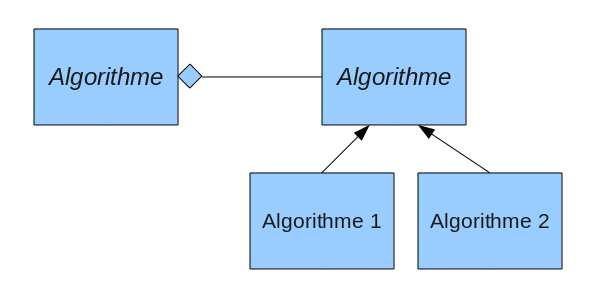
\includegraphics[width=12cm]{img/pattern-strategie.png}
	\caption{Diagramme UML du pattern stratégie}
\end{figure}

Dans notre cas, il permet de créer différents type de stratégie qui pourront potentiellement utiliser. 
Notre projet ne contenait que la stratégie "envoi de SMS" mais, avec cette architecture, il est possible 
de rajouter d'autres stratégies comme l'extinction du téléphone ou encore l'envoi d'un email par exemple.
\\


La fabrique quand à elle permet de créer des objets sans en connaitre l'éxistence avant le lancement du 
programme.

\begin{figure}[H]
	\center
	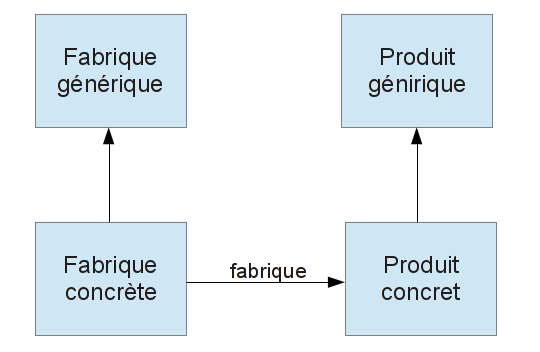
\includegraphics[width=10cm]{img/fabrique.png}
	\caption{Diagramme UML du pattern fabrique}
\end{figure}

Dans notre cas, elle permet d'utiliser de créer les stratégies et de les utiliser. En effet, la fabrique 
qui va analyser chaque nouveau message. En fonction de leurs contenus, elle devra décider d'une stratégie
et l'appliquer.


\subsubsection{Traitements des évènements}

Selon l'évènement reçu, le traitement à effectuer n'est pas le meme. Pour notre application, nous avons 
créer recensés deux évènements et traitements associés possible.

La réception d'un SMS est notre premier cas. Comme le montre le schéma ci dessous, le traitement se 
décompose en trois étapes. 

\begin{figure}[!h]
	\center
	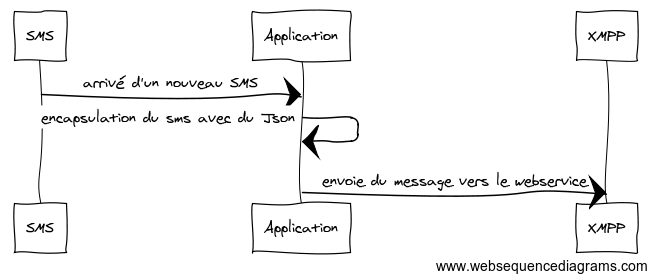
\includegraphics[width=12cm]{img/encapsulation-sms.png}
	\caption{Traitements lors de la réception d'un SMS}
\end{figure}

Il faut tout d'abord récupérer le contenu du message ainsi que son auteur. Puis il fallait encapsuler 
ses données dans un message au format Json. Enfin nous terminions par envoyer le message encapsulé vers 
le webservice qui s'occupera de notifier l'utilisateur de l'arrivé d'un nouveau message.

Concernant le deuxième évènement possible, il s'agit de la réception d'un nouveau message XMPP. Contrairement
au premier traitement, il va etre désencapsulé pour pouvoir y récupérer l'information utile. Cela fait, 
notre fabrique va s'occupper de d'appliquer la stratégie adapter pour ce nouveau message. Dans notre cas, 
puissque nous avions juste la stratégie d'envoi de SMS, c'était toujours celle-ci qui était appliqué.

%XMPP->Application: arrivé d'un nouveau message XMPP
%Application->Application: désencapsulation du Json contenu dans le message
%Application->SMS: envoie d'un SMS

\begin{figure}[!h]
	\center
	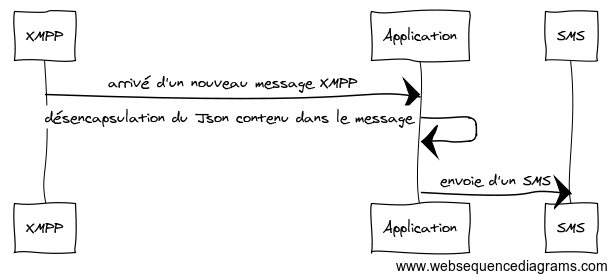
\includegraphics[width=12cm]{img/desencapsulation.png}
	\caption{Traitements lors de la reception d'un message XMPP}
\end{figure}
